\documentclass{IEEEcsmag}

\usepackage[colorlinks,urlcolor=blue,linkcolor=blue,citecolor=blue]{hyperref}

\usepackage{upmath}
\usepackage{comment}
\usepackage{graphicx}

\usepackage[usenames,dvipsnames,svgnames,table]{xcolor}
\definecolor{dkgreen}{rgb}{0,0.6,0}
\definecolor{mauve}{rgb}{0.58,0,0.82}
\definecolor{light-gray}{gray}{0.88}

\usepackage{listings}
\lstdefinestyle{agree}
{frame=none,
  basicstyle=\ttfamily,
  language=ML,
  aboveskip=3mm,
  belowskip=3mm,
  showstringspaces=false,
  columns=flexible,
  numbers=none,
  numberstyle=\tiny\color{gray},
  commentstyle=\color{dkgreen},
  stringstyle=\color{mauve},
  breaklines=false,
  breakatwhitespace=true,
  tabsize=2,
  linewidth=1.7\linewidth,
  morekeywords={eq, bool, guarantee, assume, true, false, pre, not, and, or, property, const}
}

% for diagram in synthesis.tex

\usepackage{tikz}
\usetikzlibrary{shapes}

\newcommand{\briefcase}{BriefCASE}
\newcommand{\hamr}{HAMR}
\newcommand{\selFour}{seL4}
\newcommand{\figref}[1]{Fig.~\ref{#1}}
\newcommand{\agree}{AGREE}
\newcommand{\splat}{SPLAT}
\newcommand{\resolint}{Resolint}
\newcommand{\resolute}{Resolute}

\jvol{XX}
\jnum{XX}
\paper{XX}
\jmonth{XX/XX}
\jname{Security \& Privacy}
\pubyear{2022}
\newtheorem{theorem}{Theorem}
\newtheorem{lemma}{Lemma}

\setcounter{secnumdepth}{0}

\begin{document}

%\sptitle{Department: Head}
%\editor{Editor: Name, xxxx@email}

\title{Cyber Assured Systems Engineering at Scale}
%\title{Cyber-Resilient Systems Engineering at Scale}

\author{Darren Cofer, Isaac Amundson, Junaid Babar, David Hardin, Konrad Slind}
\affil{Collins Aerospace}

\author{Perry Alexander}
\affil{University of Kansas}

\author{John Hatcliff, Robby}
\affil{Kansas State University}

\author{Gerwin Klein}
\affil{Proofcraft and UNSW Sydney}

\author{Corey Lewis}
\affil{UNSW Sydney}

\author{Eric Mercer}
\affil{Brigham Young University}

\author{John Shackleton}
\affil{Adventium Labs}

\markboth{Department Head}{Paper title}

\begin{abstract}
Formal methods tools that provide mathematical proof of system properties
have improved dramatically in their power and capabilities. Our team has developed a model-based systems
engineering environment that integrates formal methods at all levels of system design.
Our methodology and tools enable systems engineers to address
cybersecurity concerns early in the development of complex high-assurance systems.
\end{abstract}

\maketitle


%Darren, David? Budget: 1 column
%Introduction

Describe our view of the challenges and breakthroughs in the call.

Systems engineers are currently given few
development tools to help answer basic questions about
potential cyber vulnerabilities and how to  mitigate them.  Typically, they must rely on
process-oriented checklists and guidelines. Cyber vulnerabilities
are often discovered during penetration testing late in the
development process; or worse yet, they may be discovered
only after the product has been fielded, necessitating extremely
expensive and time-consuming remediation. This is not a
sustainable development model.

Fortunately, formal methods 
(define?)
has advanced to the point that new tools and techniques can 
be used to address cybersecurity and cyber-resiliency design challenges.  

Our application domain is avionics and aerospace systems in general.  
Our team has developed a model-based systems engineering (MBSE) 
envirnoment that 

scale to real aerospace systems
tools to automate capabilities that we prototyped in the HACMS project \cite{HACMS}
range of properties
complexity through composition
integration into tool environoment and language accessible by systems engineers
Ability to rapidly co-evolve systems and associated evidence; and
Ease of use for non-expert developers and evaluators.

 - Applications to specific major systems in government and industry;
 - Tour-de-force results, such as proofs of significant mathematical results or reasoning about modern processors;
 - Advancement of FM ecosystems surrounding the various provers and stacks; and

\section{INNOVATIONS}
%Darren -  Budget: 1 column
%Innovations

MBSE environment for high-assurance systems, providing access to FM tools at every level, integrating assurance evidence for co-evolving design and associated evidence.


\section{EXAMPLE}
%Eric?  Budget: 1 column
%Motivation

Introduce the phase 2 example as motivation and to illustrate the work flow to be described later. 


\section{BRIEFCASE WORK FLOW}
%Darren write a brief intro -  Budget: 0.5 column
%\cite{OSATE}
%Work Flow

%Describe the BriefCASE work flow and tools.

% Copied from DESTION paper
Our BriefCASE toolchain provides systems engineers with a workflow and tool support for developing products with inherent cyber-resiliency.
BriefCASE is predicated on an MBSE process, in which models are the primary vehicle for communication and understanding among the parties tasked with designing the system. Furthermore, MBSE models are the primary design artifacts used for analysis, verification, testing, and code generation.  

The BriefCASE workflow starts with the development of an AADL model of the system architecture. 
BriefCASE is implemented as a set of plugins that work with OSATE, the flagship tool for AADL modeling.
Once an architecture model has been created, it can be analyzed in various ways  (e.g., resource usage, information flow, latency) to determine whether the initial design is acceptable. 

BriefCASE integrates tools that analyze the architecture model for cybersecurity vulnerabilities and generate a set of requirements that, when addressed, will mitigate those vulnerabilities.  
The generated requirements are imported into the model and represented as goals in a Resolute assurance case.  As a requirement is addressed in the design, the assurance case is updated with evidence, either taken directly from the model or supporting development process outputs, necessary to support the claim.  In this manner, the assurance case is co-developed alongside the system design, and can be automatically evaluated throughout development.

\subsection{Requirements}
%Isaac, Junaid -  Budget: 1 column
%\cite{gearcase2020} \cite{dcrypps2019}
BriefCASE provides access to two analysis tools (GearCASE~\cite{gearcase2020} and
DCRYPPS~\cite{dcrypps2019}) that can examine AADL models to detect potential cyber vulnerabilities
and suggest requirements for mitigation.
%
Systems engineers are then presented with a requirements management interface
(top pane in Figure~\ref{fig:req-mgmt}) for viewing the generated requirements and importing them into the model
so they can be addressed. The interface enables engineers to select the requirements they wish to
import and assign them unique identifiers, or omit them with rationale. A document listing the omitted
requirements and rationale is maintained and may be a required development artifact for some
certification domains. 

\begin{figure*}[h]
	\centering
	\includegraphics[width=\textwidth]{figs/req-mgmt.png}
	\caption{\briefcase \ requirements management interface.} 
	\label{fig:req-mgmt} 
\end{figure*}

Some requirements can also be formalized as assume-guarantee contracts
added to the AADL model, enabling formal verification. 
Such a requirement will be imported into the model with with an associated formal
contract.

A BriefCASE project contains a repository for requirements. Imported requirements are represented in the Resolute language as assurance case goals to be satisfied. For example, one of the requirements for well-formed messages (selected in \figref{fig:req-mgmt}) is imported as the following goal:

\noindent
\includegraphics[width=1\columnwidth]{figs/req-wellformed-or.png}

% shown in \figref{fig:req-wellformed-or}.
\noindent
Initially, the goal is marked {\em undeveloped} and does not contain any evidential statements.  
These will be added as the design is updated to address this requirement.  

%for Resolute to evaluate in order to determine whether the goal has been satisfied. Running Resolute
%at this time will therefore produce a failed assurance case.

%\begin{figure}[h]
%	\centering
%	\includegraphics[width=1\columnwidth]{figs/req-wellformed-or.png}
%	\caption{Requirement for well-formed messages.  NEEDED? CONVERT TO TEXT?} 
%	\label{fig:req-wellformed-or} 
%\end{figure}

\subsection{Cyber Transforms}
%Isaac -  Budget: 1 column
To address the new cyber-resiliency requirement, the architecture will need to be transformed in such a way as to harden the design against the vulnerability.
BriefCASE provides a library of model transformations for addressing common cyber vulnerabilities.  Currently, the following transformations are supported:

% add a brief description for these?
\begin{itemize}
	\item Filter -- Blocks messages that do not conform to the given specification
	\item Monitor -- Detects violations of a given run-time condition and generates an alert
	\item Switch -- Used with a Monitor to block messages when an alert is generated (also referred to as a \textit{gate})
	\item Attestation -- Performs a measurement on non-local software to assess its trustworthiness
	\item Virtualization -- Isolates software component(s) in a virtual machine
	\item Proxy -- Inserts a pair of components to allow inspection of %https
		HTTPS message payloads
	\item seL4 -- Transforms the model to comply with seL4 component properties
\end{itemize}  

The transformations are automated by the BriefCASE tool, resulting in a hardened model that is correct-by-construction.  
For example, the requirement that a component only receives well-formed messages can be satisfied by the insertion of a high-assurance filter.  
A BriefCASE transform wizard 
% (Figure~\ref{fig:filter-wiz}) 
helps to configure the filter component properties, including the filter behavioral specification, which is represented as an assume-guarantee contract.

%\begin{figure}[h]
%	\centering
%	\includegraphics[width=0.8\columnwidth]{figs/filter-wiz.png}
%	\caption{Filter transform wizard.} 
%	\label{fig:filter-wiz} 
%\end{figure}

BriefCASE then inserts a new filter component into the model, sets the component properties, and establishes the appropriate connections to source and destination components. The filter behavioral contract is also added to the model, enabling formal analysis of the model as well as providing the behavioral specification for a provably correct synthesis of the filter component implementation.

The transformation also updates the assurance case with new evidential statements indicating that the associated goal has been satisfied, including 
the strategy used and links to context and associated evidence.  

%(as shown in Figure~\ref{fig:resolute-add-filter}).
%For example, the \texttt{add\_filter} strategy is included in a library of built-in Resolute transform rules and provides Resolute with the logical instructions for evaluating if the top-level goal has been satisfied.
%The \texttt{add\_filter} definition (shown in Figure~\ref{fig:resolute-add-filter}) includes the following sub-goals: 
%\begin{itemize}
%	\item \texttt{filter\_exists} - the filter component exists in the model
%	\item \texttt{filter\_not\_bypassed} -  there is no alternate pathway in the model that can bypass the filter
%	\item \texttt{filter\_implemented\_correctly} - the filter has been implemented correctly
%\end{itemize}
%
%
%\begin{figure}[h]
%	\centering
%	\includegraphics[width=1\columnwidth]{figs/resolute-add-filter.png}
%	\caption{Updated well-formedness claim.} 
%	\label{fig:resolute-add-filter} 
%\end{figure}

%The first two sub-goals are supported by evidence obtained by examining the structure of the model, while the last is determined by examining the output of the synthesis tool.  
%%This approach follows the model-based decomposition pattern based on~\cite{model-based-decomposition}, and is representative of all BriefCASE transform assurance strategies.
%If at a later time during development the model is inadvertently altered in a way that renders the transformation ineffective, Resolute will be unable to substantiate the evidential statements, and therefore produce a failing assurance case.
%
%The third subgoal is satisfied by SPLAT.  SPLAT not only generates the  implementation code for high-assurance components such as filters, monitors, and gates, but it also produces a proof that this code correctly implements its AGREE specification.  
%Resolute uses the existence of the SPLAT proof as evidence that the component was implemented correctly.


\subsection{Compositional Analysis}
%Junaid -  Budget: 1 column
%\cite{case-models-2021}
% Compositional Analysis

Once the system's architecture has been modeled using AADL
and component behavior specified using \agree's assume-guarantee contracts,
we use \agree's model checker to verify the consistency of these contracts.
The model checking process verifies that:
(a) the output guarantees of component implmentations are strong enough to
validate the input assumptions of downstream components; and 
(b) the input assumptions of a component along with the output guarantees of its \emph{sub}-components
are strong enough to validate its output guarantees.
For example, in \figref{fig:sw-hardened},
the input assumptions of the Waypoint Manager must be inferrable from
the output guarantees of the Geofence monitor, 
and the output guarantees of SW must be inferrable from
its input assumptions combined with the output guarantees of its subcomponents.

This hierachical strategy for reasoning about contracts,
i.e. \emph{Compositional Analysis},
reduces the computational complexity of model checking
by breaking down the larger problem into more manageable fragments \cite{compositional-analysis-agree}.
In \figref{fig:sw-hardened}, SW's subcomponents can be broken into further subcomponents,
and this would, typically, multiply the complexity of the verification process.
But, in the case of Compositional Analysis (and \agree),
since verification of a component does not (directly) depend on the contracts of its \emph{sub}-subcomponents,
this multiplication of complexity does not occur.
More details can be found in \cite{case-models-2021}.


\subsection{High Assurance Component Synthesis}
%% Konrad, Eric, Junaid -  Budget: 1 column
%% \cite{case-verified-filter} \cite{hardin-co-assurance}
%% \cite{formal-filter-synth-langsec} \cite{contiguity-types}
The correctness of the leaf-level components introduced by CASE
transformations resolves to the question of whether such a component
meets its AGREE contract. This proof obligation is approachable in
various ways: for example, it can be dealt with by inspection, unit
testing, or by formal proof. In CASE, we take a version of the formal
proof route: \emph{synthesis}. In particular, given a sufficiently
detailed formal contract, we generate code from it and generate proofs
showing that the generated code obeys the contract.

The formal languages that filters, gates, and monitors are generated
from include regular expressions, \cite{case-verified-filter},
contiguity types \cite{contiguity-types}, and Lustre. For each of
these languages, we have infrastructure (see Figure
\ref{fig:synthesis} that (a) translates formal specifications to code
and (b) proves the correctness of the translation. The generated code
is CakeML \cite{cakeml}, a verified compiler for a Standard ML
variant.

\begin{figure}[h]
\begin{center}
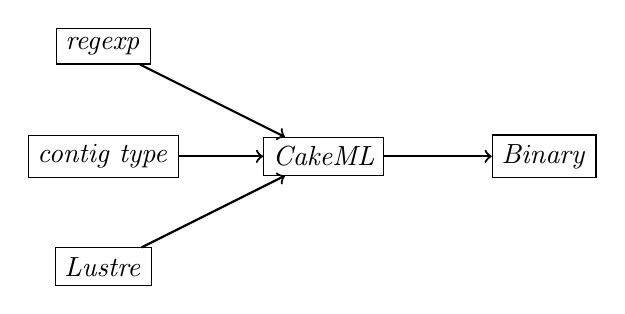
\begin{tikzpicture}[scale = 0.7]
\node (A) at (0,2) [shape=rectangle,draw]{\textit{regexp}};
\node (B) at (0,0) [shape=rectangle,draw]{\textit{contig type}};
\node (C) at (0,-2) [shape=rectangle,draw]{\textit{Lustre}};
\node (D) at (4,0) [shape=rectangle,draw]{\textit{CakeML}};
\node (E) at (8,0) [shape=rectangle,draw]{\textit{Binary}};
\draw [->,thick] (A) to (D);
\draw [->,thick] (B) to (D);
\draw [->,thick] (C) to (D);
\draw [->,thick] (D) to (E);
\end{tikzpicture}
\end{center}
\caption{Synthesis path.\label{fig:synthesis}}
\end{figure}


\subsection{Remote Attestation}
%Perry -  Budget: 1 column
%\cite{copland-attestation} \cite{copland-verification}
Semantic remote attestation is a technique for remotely establishing
trust in running software.  An appraiser requests an attestation from
a target, receives evidence in response it the request, and appraises
the evidence to determine
trust~\cite{Haldar:04:Semantic-Remote,Coker::Principles-of-R}. Because
remote attestation does not require modification of its measurement
target, StairCASE utilizes it to establish trust in legacy software
that cannot otherwise be verified.  We construct a verified remote
attestation infrastructure around the legacy target that generates
run-time and boot-time evidence.

The approach adds three attestation managers to the seL4-based
architecture used to harden the attestation target.  Each attestation
manager executes protocols specified by Copland~\cite{Ramsdell:2019aa}
phrases.  Copland is a formally specified language designed for
writing attestation protocols that are both verifiable and executable.
The attestation managers themselves are written and verified using
CakeML~\cite{Kumar:2014:CVI:2535838.2535841} and
Coq~\cite{Bertot:2013aa}.

The UserAM runs as a Linux process on the seL4 virtual machine.  It's
responsibilities are responding to attestation requests from off
platform, measuring the hardened application, and requesting
attestations from the platform.  When the UserAM receives an
attestation request it responds by executing an attestation protocol
that measures the hardened application, requests measurements from the
PlatformAM, and signs the result and a nonce from the request.  The
resulting evidence package is returned to the requesting appraiser.

Because the UserAM runs as a process in the Linux kernel, it cannot be
trusted \emph{a priori}.  A PlatformAM is introduced to perform an
attestation on the Linux kernel.  The PlatformAM runs as a
CAmkES component separated from the Linux kernel.  seL4's guaranteed
separation properties provide assurance that the PlatformAM cannot be
interfered with by other platform software.  The PlatformAM only
responds to requests from the UserAM and similarly runs a protocol
that produces signed results.

A third attestation manager is added to the appraiser to make
attestation requests and appraise results.  A protocol and nonce are
sent to the target, evidence is returned, and results appraised to
determine trust.  The attestation manager then communicates appraisal
results to the platform communicating with the remote target.  In this
way the platform appraises a remote target before trusting it to
behave as expected.

Using the remote attestation system to harden a platform involves
writing application specific attestation and appraisal components.
New measurers are constructed for the UserAM that measure the running
application along with corresponding appraisal code.  The PlatformAM
and attestation architecture remain the same across applications.  The
overhead required for hardening is thus minimized.

\subsection{Information Flow Analysis}
\label{subsec:info-flow}
%Robby -  Budget: 1 column

As systems become more complex, composition of components and 
systems presents safety and security challenges that span
many sub-systems.  Subsystems and components may originate from
different organizations -- many of which may not have a complete
understanding of system information flows and potential impacts of
security attacks.  Thus, it is essential to have trustworthy methods
of developing common understanding of dependencies in the system and
the respective responsibilities of the involved vendors.  On CASE, the
Awas~\cite{awas} AADL information flow analyzer and visualizer has been 
applied to enable allow developers and auditors to understand, reason,
explore, and visualize system dependencies and information flow at
scale across components and sub-systems.  Awas processes the AADL
system architecture model, specifically its inter-component connection
descriptions and intra-component flow specifications, to provide
formal system-wide impact and flow analyses.
Such flows include component data/control flows,
security-oriented information flows, and fault/error propagation
specified using by the AADL Error Modeling Annex (EMv2).
Awas also provides a user-friendly Domain Specific Language (DSL) to 
query, check, and visualize custom safety/security system properties.

\begin{figure}[h]
	\centering
	\includegraphics[width=\columnwidth]{figs/CASE-Awas.png}
	\caption{CASE Awas Information Flow Analysis.} 
	\label{fig:CASE-Awas} 
\end{figure}

Figure~\ref{fig:CASE-Awas} illustrates an example of Awas information flow reachability analysis.
From a given component or port (e.g., an output port of the Ground Station),
Awas can compute and visualize how the Ground Station’s map information flows through the system
as well the components/ports that may directly or indirectly consume data derived from that information.
Awas supports a number of forms of forwards and backward interactive information queries.
Using the Awas script-based query language, one can specify and check more complex properties, e.g.,
that information must flow through specific ports or components.
These end-to-end flow specifications are often useful for supporting verification of the
effectiveness of cyber-resiliency components.   For example, an Awas specification can state that
information from untrusted components such the Ground Station always flow through the
attestation gate and filter components before reaching the Flight Control or other components
that make critical decisions about the flight or mission of the UAV.

The HAMR code generation and associated formally verified information
flow correspondence evidence described subsequently
%%described in Section~\ref{subsec:hamr}
guarantees that the seL4 microkernel is configured to permit the exact
inter-component information flows analyzed and visualized by Awas at
the model level.

\subsection{Real-Time Scheduling}
%John S -  Budget: 1 column
% Real-Time Scheduling

\it{temporal isolation} is a technique to reduce timing channels and temporal 
interference between software threads executing on the same platform. 
In certain conditions,
timing channels can be used to violate confidentiality requirements. 
Temporal interference can reduce availability of time-critical functionality, 
and impact integrity of controls by inducing selective jitter. 
For example, if one component is compromised, it could dominate the processor, 
preventing other components from completing their tasks, placing the security 
of the entire platform in jeopardy. 
In mixed-criticality mission systems, 
multiple threads necessary for mission success often 
have strict confidentiality, integrity, and availability requirements. 
Simple scheduling approaches that attempt to use priority schemes to mitigate 
this impact only protect the highest priority threads.

\briefcase\ achieves \it{temporal isolation} in a real-time
environment in which threads execute within
their own scheduled timing constraints without interference from other
threads hosted on the same platform. To accomplish this, we leveraged
prior work from safety and security-critical disciplines, such as
avionics, where temporal isolation in real-time scheduling has been
deployed for decades. We implemented a static cyclic scheduling
approach using the \selFour\ domain scheduler, where a fixed schedule
defines an ordered sequence of static execution slots. Each slot has a
duration and a partition identifier.  \selFour\ ensures that the
temporal domain, and any threads running in it, will not exceed their defined
time allotments. Creation of a valid static cyclic schedule that
satisfies all the application's timing requirements is the
responsibility of the system designers.

\briefcase\ generates a start-of-frame synchronization signal for each thread using
a special thread called the Pacer, which sends periodic signals
to each thread. Each application thread blocks until it receives its
signal from the Pacer. The thread runs to complete, and then
blocks again on the Pacer signal for the next iteration. 
Each thread subsequently executes
exactly once during its statically scheduled time slice.

The new \selFour\ Mixed-Criticality Systems (MCS) variant provides
additional capability that can support temporally isolated
real-time systems. 
As part of \briefcase\ we developed a proof-of-concept static cyclic
scheduler for MCS.
It includes a start-of-frame signal, which
eliminates the need for the Pacer component. It also includes kernel
level support for flexible dynamic scheduling that satisfies some
real-time properties, such as period and execution time.



\subsection{Infrastructure Code Generation}
% John H -  Budget: 1 column
\label{subsec:hamr}

%% Text for the Infrastructure Code Generation subsection
% - assigned to John Hatcliff

The High Assurance Modeling and
Rapid engineering for embedded systems tool (\hamr)
\cite{hamr} is a multi-platform, multi-language
AADL code generation framework.  In the CASE project, HAMR is primarily used
to generate code for deployment for the seL4 microkernel, but system and component
prototyping is also supported utilizing HAMR's code generation capability
for the Java Virtual Machine (JVM) and Linux.  

Using seL4 as a foundation, HAMR enables
AADL to be used as a model-based development and systems
engineering framework for seL4-based applications.
One of the primary objectives is to support system builds that
leverage seL4 separation and information flow
guarantees to achieve the AADL-specified component isolation and
inter-component communication needed for cyber-resiliency.
HAMR ensures that seL4 is configured to permit the exact
inter-component information flows analyzed and visualized by Awas at
the model level.

For each AADL thread component, HAMR generates a thread code
skeleton and application programming interfaces (APIs) for communicating over the ports declared on
the component.  For components that are implemented manually, the
developer fills out the thread skeleton with application code.
\remove{,
calling the port APIs, libraries, and component-specific
developer-implemented support code as needed.}
HAMR supports coding component application logic in either C,
Slang~\cite{slang} (a high-assurance subset of Scala that can be translated to
C), or CakeML. 
\remove{
Slang-implemented components can interface with
Scala or Java libraries and execute on the JVM.  Pure Slang
components can be translated to C and then deployed on HAMR-built
Linux or seL4 systems.  On CASE, Slang has been used for prototyping
components, but primary development of directly implemented
components has used C.
For high-assurance components specified
using SPLAT, HAMR automatically integrates code generated from
SPLAT into the component binary code using CakeML's Foreign
Function Interface (FFI) mechanism.}

HAMR generates component infrastructure and integration code
implementing the semantics of AADL-compliant thread scheduling,
thread dispatching, and port-based communication.
For port communication, shared memory communication (AADL
data ports), buffered messaging (AADL event data ports), and
buffered notification (AADL event ports) are supported.
HAMR code generation is staged using a translation architecture
that facilitates adding new backends for different target
platforms.   Almost all the infrastructure code is implemented
in Slang, which can then be used for JVM deployments or
translated to C for Linux or seL4 deployments.
The Slang-based implementation of the AADL run-time framework
can be viewed as a high-level reference implementation of AADL
semantics.   Automatic translation of this reference
implementation to C on different platforms helps establish
semantic consistency across those platforms. 
\remove{The AGREE contract language and SPLAT
code generation framework have been designed to align with the AADL
semantics reflected in this reference implementation.}

The seL4 deployment uses the component architecture for microkernel-based embedded systems
(CAmkES) code-generation framework to configure the microkernel.
The HAMR generated CAmkES directly encodes the AADL model's component and communication
topology and includes the AADL run-time infrastructure with its thread scheduling.
HAMR leverages the existing seL4 domain scheduler to enforce time partitioning and provide static cyclic scheduling.

HAMR additionally supports Linux-based virtual machine components in the seL4 deployment and the ability to run the entire system on the QEMU emulator.
HAMR automatically configures virtual machine based components, and this feature is used to sandbox the untrusted legacy code for the Mission Planner in the example UAV system.
The QEMU emulator support facilitates rapid prototyping for test, debug, and analysis, and it enables automated regression testing.

\remove{To generate deployments on seL4, HAMR makes use of the
component architecture for microkernel-based embedded systems
(CAmkES) code-generation framework. The CAmkES input
language supports specification
of seL4 partitioning and communication topology using
component-oriented idioms.  
The CAmKES translator generates an
seL4 \emph{Capability Description Language (CapDL)} file that
configures the seL4 kernel to support protected memory blocks
and permission-based reading and writing of each block as
indicated by CAmkES components and connections.
To realize the memory separation specified by the AADL
architecture description, HAMR generates CAmkES specifications
that: (a) reflect the AADL model's component and communication
topology, and (b) include additional components and communication
to support the AADL run-time infrastructure, in particular,
thread scheduling.
To enforce time partitioning, HAMR uses the seL4 domain
scheduler to support static cyclic scheduling. 
}

\remove{HAMR also provides automated support for configuring Linux-based
virtual machines as components within the seL4 deployed system. 
In the example UAV system, this feature has been used to sandbox untrusted legacy code
for the Mission Planner component.}

%In CASE workflows,
%the FASTAR AADL scheduling tool from Adventium Labs was used
%to generate a candidate static schedule, and then the schedule
%was adjusted as needed based on timing experiments (this was
%needed primarily for VM components).

\remove{HAMR-generated seL4 systems can be executed on the QEMU emulator
before deployment to a development board or
production hardware.  This prototyping capability significantly speeds up development
iterations and enables the development of a sophisticated
automated regression testing framework.}

\remove{While we have not yet completed full formal verification of
the HAMR Slang-based reference implementation and code generation
pipeline, information flow preservation is a key property that 
illustrates how one might approach formal verification of 
other important semantic properties.
Specifically, }

HAMR generates flow graphs reflecting the inter-component information flow at both the AADL architecture level and the CAmkES level for the seL4 deployment.  
These are both visualized for manual inspection and given SMT-based representations for formal reasoning.
The SMT-based representations are used to prove the following:

\remove{In addition to multiple visualizations and traceability artifacts that can be audited, HAMR
generates SMT-based representations of the flow graphs and
traceability relationships between them.  Formalized
theorems for information flow preservation can then be represented as
SMT assertions.  This enables SMT solvers to automatically prove
the following properties for any HAMR-generated seL4 deployment:
}

\begin{enumerate}
\item The modeled flows are in the CAmkES. \remove{All AADL flows are implemented -- For every inter-component information
flow present in the AADL model, that flow is provisioned in the
generated seL4 kernel configuration.}
\item No extraneous flows are in the CAmkES.\remove{ -- For
each inter-component flows provisioned in the seL4 kernel, that
flow is represented as an inter-component connection in the
AADL model.}   
\end{enumerate}
These properties focus on
cyber-resiliency, but other
key semantic properties can be verified as well.
\remove{ e.g., by applying the Slang Logika formal
verification capability to the Slang reference implementation of the
AADL run-time.}  

\remove{
HAMR plays a key role in integrating formal methods
at different levels of abstraction at multiple points throughout
the development process, enabling those methods to be applied
at-scale in the system development process.   Using the
formally verified seL4 microkernel as a foundation, HAMR enables
AADL to be used as a model-based development and systems
engineering framework for seL4-based applications.
HAMR provides a semantically-consistent multi-platform code
generation process that enables: (a) formally verified components
(e.g., generated from SPLAT) to be correctly integrated and
deployed; and (b) formal specification and verification frameworks
like AGREE to be used to reason about both component and system
level properties.   The HAMR code generation architecture is
designed to support strong traceability and verification, as
illustrated by the information flow correspondence properties.  
The compositional and staged nature
of HAMR-based development supports scaling of formal approaches
by enabling them to be included in a component-wise manner and at
different levels of abstraction, while
also integrating parts of the implementation that are assured
using traditional methods.   In addition, the strong partitioning
of seL4 enables the controlled integration of untrusted components.
}

%SOME OF THIS LAST PARAGRAPH MIGHT BE BETTER IN THE CONCLUSION.




\subsection{Secure Microkernel}
% Corey, Gerwin -  Budget: 1 column
% word budget: ~ 400 words

The seL4 microkernel is a lightweight, fast, and secure operating system (OS) kernel.
Its implementation is fully formally verified; from high-level security properties
down to the binary level~\cite{sel4-formal}. It was the first OS kernel with this
degree of formal verification, and after more than a decade of further research
and engineering is still not only the leading formally verified OS kernel, but also
the fastest OS kernel on the Arm architecture.

Its formal verification makes seL4 the ideal basis for high-assurance systems.
It is in itself a demonstration of the level of fidelity and scale formal
verification can achieve. It supports multiple architectures (Arm, x86-64,
RISC-V), deep security properties such as integrity, confidentiality and
availability, and comes with formally verified user-level system initialization.
As one of its multiple available OS personalities, it also offers a user-level component
system that provably achieves isolation between statically specified components.

The formal proofs about seL4 and the corresponding user-level components measure
over one million lines of proof script in total. They constitute one of the
largest continually maintained formal proof artifacts in existence and provide a
rich target for new techniques in proof engineering, proof repair, and
automation for constructing new proofs about software as well as maintaining
existing large-scale proof artifacts.

While it is essential to build a high-assurance system on a high-assurance OS
kernel, this is not the main feature seL4 provides for systems engineering --- a
simpler real-time OS might be formally verified, but would not be sufficient for the
engineering method described in this paper. The true power of seL4 lies in its
ability to scale formal analysis and verification to the much larger code bases
that make up entire systems. It does so by providing strong isolation between
user-level components.

This isolation means that components can be analyzed separately from each other
and be composed safely --- in this way seL4 provides the foundation that the soundness of the highly
automated analysis tools such as AGREE depend on. It makes it possible to run
entire untrusted virtual machines and securely monitor their behavior on the
same hardware. It makes it possible to provide filter and monitor components and
prove that these components cannot be tampered with by the components they protect.
It makes it possible to guarantee that the limited communication channels that the analysis tools
use on are the \emph{only} communication channels that are available to the
components in the system.


\subsection{Assurance Case}
%Isaac -  Budget: 1 column
An important aspect of our work has been to structure formalizations and proofs by following
the AADL model of the system. 
%In other work, we did this through the use of formal
%assume-guarantee contracts that correspond to the requirements for each component~\cite{HACMS}. 
We have found that in assuring the cyber-resiliency properties of aircraft designs we need to integrate
different kinds of evidence with varying levels of formality. This has been our motivation to
explore assurance case methods.

In previous work, we developed the {\em Resolute} language and
tool~\cite{resolute2014},~\cite{resolute-destion} as a way to help developers create an assurance
argument describing the steps taken during the design process to make the system safe and secure.
The Resolute syntax supports construction of assurance cases that comply with the Goal Structuring
Notation (GSN) v2 standard~\cite{GSNv2}. Claims are expressed as \textit{goals} and
\textit{strategies}, and can contain attributes such as \textit{context}, \textit{assumptions}, and
\textit{justification}. Claims can be marked \textit{undeveloped}, which Resolute interprets as an
unsupported claim, or with a \textit{solution}, which is an explicit assertion that the claim is
supported. Rather than being a separate document, a Resolute assurance case is part of the
architecture model and can refer to elements within the model. Since it is not a static
representation, it can ensure that the assurance argument remains consistent with the evolving
design.

BriefCASE includes a library of Resolute assurance strategies, or \emph{patterns}, that align with
the CASE workflow. The patterns are instantiated with context from the AADL model and specify the
evidence required to support the cyber-resiliency goals of the system. For example, the
\texttt{add\_filter} strategy is automatically inserted into the assurance case when the
\textit{Filter} transformation is performed, and includes logical rules that Resolute uses to
determine whether the well-formedness claim is supported by evidence. The \texttt{add\_filter}
definition 
%(shown in Figure~\ref{fig:resolute-add-filter}) 
includes the following sub-goals:
\begin{itemize} 
\item \texttt{filter\_exists} -- The filter component is still present in the model and has not be 
altered or deleted by subsequent design changes. 
\item \texttt{filter\_not\_bypassed} -- There is no alternate information flow in the model that 
would allow the filter to be bypassed and therefore not perform its function.   
\item \texttt{filter\_implemented\_correctly} -- The filter has been implemented correctly 
to meet its AGREE specification.  
\end{itemize}

\begin{figure}[h] 
\centering 
\includegraphics[width=1\columnwidth]{figs/resolute-add-filter.png}
\caption{Updated well-formedness claim. REPLACE WITH ASSURANCE CASE DIAGRAM?}
\label{fig:resolute-add-filter} \end{figure}

The first two sub-goals are supported by evidence obtained by examining the structure of the model. 
If at a later time during development the model is inadvertently altered in a way that renders the transformation
ineffective, Resolute will be unable to substantiate the evidential statements and will
produce a failing assurance case.

The third subgoal is satisfied through the use of SPLAT. SPLAT not only generates the implementation code for
high-assurance components, but it also produces a proof that the generated code correctly 
implements its AGREE specification. Resolute uses the existence of the
SPLAT proof correlated with the model revision number for the AGREE specification
as evidence that the component was implemented correctly.


% Resolute can determine whether an assurance case passes or fails


% Advocate?

% Show generated assurance case (in Advocate?)

\section{AIRCRAFT APPLICATION}
%David -  Budget: 1 column
We have successfully demonstrated our BriefCASE methodology and tools to
develop proof-of-concept enhancements for the CH-47F helicopter Common Avionics
Architecture System (CAAS). As an integrated cockpit avionics suite developed by Collins Aerospace, CAAS serves
as a prime example of modern air platform complexity with common avionics across a variety of
defense platforms including the Army's Mission Enhanced Little Bird (MELB)  and MH-60, the
Navy CH-53K, and the Air Force KC-135. The CAAS application offered an opportunity to
apply BriefCASE tools across a variety of mission systems, including legacy components, flight critical
software, as well as new and evolving systems. 
%As the primary designer and manufacturer of CAAS,
%Collins Aerospace maintains complete design artifacts including boot loaders, operating systems,
%software applications, hardware, and bus message specifications. 

Most of the work for this demonstration was 
performed by a team of CAAS development engineers who had no
previous experience with formal methods.
Our primary goal was to enable CAAS product engineers to employ the CASE tools to create an
operational mission scenario exhibiting cyber threats and mitigations that could be exercied using
the facilities of the Collins CH-47F System Integration Laboratory. 

\begin{figure*}
	\begin{center}
	\includegraphics[width=\textwidth]{./figs/caas-arch.png}
        \end{center}
	\caption{Cyber-resilient software architecture adding wireless device access to CH-47 avionics.} 
	\label{fig:caas-arch} 
\end{figure*}

The CH-47F demonstration system
for CASE focused on integrating pilot and soldier wireless tablet computers for
increased situational awareness and display of Automatic Dependent Surveillance-Broadcast (ADS-B)
data regarding nearby air traffic (\figref{fig:caas-arch}).  
BriefCASE tools were used to implement this networking enhancement while ensuring that no new cybersecurity
vulnerabilities were introduced.  A high-assurance gateway was added between the existing CAAS 
network and the new wireless network, including new components for monitoring messages to and from the wireless 
devices.  Remote attestation was also added to ensure that any devices that attempt to join the wireless network
are running trustworthy software.   
This also required porting the seL4 microkernel to an existing CAAS
processing module (the vision processing module, or VPM) that would be repurposed to serve as the secure gateway.  

%This vision processing module, or VPM, is provisioned to allow only vetted
%traffic to/from the aforementioned wireless clients in order to provide situational awareness data
%to pilots and soldiers, as well as to provide a platform for the execution of CASE-tool-generated
%filters, monitors, attestation gates, etc.

The CAAS engineers first developed an AADL model of the CH-47F CAAS system. They added the
enhanced capabilities for wireless access described above, resulting in a baseline architecture. The 
engineers then analyzed their baseline AADL architecture utilizing the GearCASE and DCRYPPS tools,
resulting in a set of cyber requirements. They employed the BriefCASE AADL tools to add
filters, monitors, attestation gates, and seL4 isolation to satisfy the cyber
requirements. ADS-B anti-spoofing monitors were also developed by the CAAS team to 
detect inconsistencies in aircraft position and velocity trends,
bad traffic identifiers, and other possible indicators of spoofed aircraft.

The specifications for the filters and monitors were developed by the CAAS engineers
using the AGREE contract language, with assistance from our research team.  The SPLAT tool was
used to synthesize the monitors and filters from the AGREE specifications
with high assurance, as described above. The HAMR tool was then used
to generate infrastructure code for the overall system running on seL4.
%including the seL4 CAmkES components, CAmkES I/O, the processing schedule, etc.

The tablet operating environment was modified to run application software in a Linux virtual machine
hosted on seL4.  This was necessary to add the remote attestation components.  

%utilized either an off-the-shelf Android environment, or a Linux
%guest OS running on seL4. This provided the CASE remote attestation team with differing challenges
%when it came to the measurement and attestation of the tablet platform types, and provided the CASE
%independent evaluators a variety of options for formulating attacks against the system. The ADS-B
%anti-spoofing monitor developed by the CAAS team detected position/velocity trend inconsistencies,
%duplicate traffic identifiers, as well as ``teleporting'' aircraft.

The port of the seL4 microkernel to the VPM was complicated by the need for network
proxy and adapter components to bridge the untrusted wireless network to the rest of the sytem in a trustworthy
manner, including the ability to filter encrypted network traffic payloads. Fortunately, dedicated
processing cores were available on the VPM for the provisioning of these ``low-side'' and ``high-side''
components. This code had to be manually written due to the complexity of dealing with
off-the-shelf networking technologies.  Automating the synthesis of network adapter and proxy components
is future work.

As initial users of the BriefCASE tools, the CAAS engineers encountered some limitations in the
specification expressiveness and documentation, as might be
expected for the first use of a research tool suite by product area developers. 
This led to improvements in the tools to add or extend capabilities.  Initial estimates of
processing time required for the complex monitoring components turned out to be optimistic,
requiring an optimization effort. Lack of detailed seL4 support for the target hardware led to more
extensive porting efforts for the VPM and tablets than was originally anticipated, and tablet
hardware instabilities further hampered the porting effort. But all in all, the CASE tools were able
to be productively used by Collins product area engineers to produce the CH-47F CAAS demonstration
system on time and within budget, providing our research team with valuable feedback on the
strengths and weaknesses of the current BriefCASE tool envionment.



\section{CONCLUSION}
% Budget: 0.5 column
%The manuscript should include a conclusion. In this section,
%summarize what was described in your paper. Future directions may
%also be included in this section. Authors are strongly encouraged not
%to reference multiple figures or tables in the conclusion; these
%should be referenced in the body of the paper.
We have produced a model-based systems engineering environment
called BriefCASE, based on the Architecture Analysis and Design
Language.  The BriefCASE tools and methodology provide design, analysis, and code
generation capabilities based on formal methods and targeted at
high-assurance cyberphysical systems.  

Key innovations include automated architectural design patterns 
for cyber-resiliency, co-evolution of system design and assurance 
artifacts (captured as an assurance case linked to the architecture model), 
synthesis of code for high-assurance components, and code generation
targeting the formally verified seL4 microkernel.  

We have demonstrated the effectiveness and scalability of these 
tools by using them to add new cyber-resilient features to a military 
helicopter avionics system.  Their successful use by our product engineers 
provides evidence that formal methods can be incorporated into 
industrial projects.  

All of the tools are open-source, with links and documentation available
at \url{http://loonwerks.com/projects/case.html}.  We hope that others 
will find value in this approach and extend the tools with new cyber transforms, 
expanded system analysis tools, and code generation for additional operating 
systems and computing platforms.  







%BriefCASE provides
%access to two cyber requirements analysis tools (GearCASE
%and DCRYPPS) that can examine AADL models to detect potential
%cyber vulnerabilities and suggest requirements for mitigation.
%A library of architectural transforms guides systems engineers
%through automated model transformations that modify the
%architecture to address these requirements, oftentimes inserting new
%high-assurance components synthesized from formal
%specifications using the SPLAT tool. Formal verification that the
%transformed system model satisfies its cyber requirements is accomplished
%via model checking using the Assume Guarantee Reasoning
%Environment (AGREE). Cyber-resilient code implementing the
%verified model is automatically generated using the HAMR
%tool. If desired, this code can be targeted to the formally
%verified seL4 secure microkernel.  Another novel aspect of our approach is
%the use of an assurance argument embedded in the architecture model
%itself to capture and document the design decisions made during this
%process, along with associated rationale.
%
%We have successfully demonstrated our BriefCASE methodology and tools on the
%CH-47F helicopter Common Avionics Architecture System (CAAS), utilizing a team of CAAS
%development engineers who had no previous experience with formal methods.  We
%are currently incorporating lessons learned from this experience to improve the BriefCASE
%methodology and tools, focusing on scalability and usability.


%open-source, prototype, extensible to other domains
%link to loonwerks.com
%significance -- recap innovations, scale, accessibility
%application to real systems

\section{ACKNOWLEDGMENT}

This work was funded by DARPA contract HR00111890001. The
views, opinions and/or findings expressed are those of the authors
and should not be interpreted as representing the official views or
policies of the Department of Defense or the U.S. Government.

\bibliographystyle{IEEEtran}
\bibliography{biblio}

\begin{IEEEbiography}{Darren Cofer}{\,}is a Fellow at Collins Aerospace. His research interests include formal methods and tools for verification and certification of high-integrity systems. He received his PhD in Electrical and Computer Engineering from the University of Texas at Austin and is a senior member of the IEEE. Contact him at cofer@ieee.org.
\end{IEEEbiography}

\begin{IEEEbiography}{Isaac Amundson}{\,}is a research engineer at Collins Aerospace, focusing on MBSE, formal verification and assurance.  He received his PhD in Computer Science from Vanderbilt University.
\end{IEEEbiography}

\begin{IEEEbiography}{Junaid Babar}{\,}is a researcher at Collins Aerospace.
\end{IEEEbiography}

\begin{IEEEbiography}{David Hardin}{\,}is a Chief Technologist in the Applied Research and Technology organization of Collins Aerospace.  Dr. Hardin has made contributions in the areas of formal methods, high-assurance computer architecture, and real-time embedded Java, and is the editor of the book \emph{Design and Verification of Microprocessor Systems for High-Assurance Applications}.  He received his PhD in Electrical and Computer Engineering from Kansas State University.
\end{IEEEbiography}

\begin{IEEEbiography}{Konrad Slind}{\,} (PhD, TU Munich) is an industrial logician at Collins Aerospace.
  His research interests include design and implementation of higher
  order logic theorem provers, verified compilation, and
  self-describing data formats,
\end{IEEEbiography}

\begin{IEEEbiography}{Perry Alexander}{\,}is the AT\&T Foundation
  Distinguished Professor and Director of The Information and
  Telecommunication Technology Center at The University of Kansas.
  His research interests include trusted computing, remote
  attestation, formal verification and formal synthesis. He received
  his PhD from The University of Kansas.
\end{IEEEbiography}

\begin{IEEEbiography}{John Hatcliff}{\,}
\end{IEEEbiography}

\begin{IEEEbiography}{Robby}{\,}
is a Professor of Computer Science at Kansas State University working
in the area of formal methods, software engineering, and programming
languages.
%%He received his PhD in Computer Science from Kansas State University.
He received a NASA Turning Goals Into Reality award in 2003,
a NSF CAREER award in 2007, an ICSE 2000 Most Influential Paper award in 2010,
and an ACM SIGSOFT Impact award in 2010.
\end{IEEEbiography}

\begin{IEEEbiography}{Gerwin Klein}{\,}
is Chief Scientist at Proofcraft and Conjoint Professor at UNSW Sydney. His
research interests include software verification, semantics of programming
languages, and proof engineering. He is the architect of the seL4 microkernel
verification which received the SIGOPS Hall of Fame Award. He received his PhD
in Computer Science from TU Munich.
\end{IEEEbiography}

\begin{IEEEbiography}{Corey Lewis}{\,}
\end{IEEEbiography}

\begin{IEEEbiography}{Eric Mercer}{\,}
\end{IEEEbiography}

\begin{IEEEbiography}{John Shackleton}{\,}
  is a Senior Principal Research Scientist at Adventium Labs,
  focused on real-time embedded systems, cybersecurity, and
  model-based system engineering and analysis.
\end{IEEEbiography}

Author's latest degree received or which he/she is currently pursuing
(He received the B.S. degree and the M.S. degree...."). Author's
research interest. Association with any official journals or
conferences; major professional and/or academic achievements, i.e.,
best paper awards, research grants, etc.; any publication information
(number of papers and titles of books published). Author membership
information, e.g., is a member of the IEEE and the IEEE Computer
Society, if applicable, is noted at the end of the
biography. Biography is limited to single paragraph only (He is a
member of IEEE, etc.). All biographies should be limited to one
paragraph, five to six sentences


\end{document}
